\PassOptionsToPackage{unicode=true}{hyperref} % options for packages loaded elsewhere
\PassOptionsToPackage{hyphens}{url}
\PassOptionsToPackage{dvipsnames,svgnames*,x11names*}{xcolor}
%
\documentclass[
  a4paper,
  twoside]{article}
\usepackage{lmodern}
\usepackage{amssymb,amsmath}
\usepackage{ifxetex,ifluatex}
\ifnum 0\ifxetex 1\fi\ifluatex 1\fi=0 % if pdftex
  \usepackage[T1]{fontenc}
  \usepackage[utf8]{inputenc}
  \usepackage{textcomp} % provides euro and other symbols
\else % if luatex or xelatex
  \usepackage{unicode-math}
  \defaultfontfeatures{Scale=MatchLowercase}
  \defaultfontfeatures[\rmfamily]{Ligatures=TeX,Scale=1}
  \setmainfont[]{Verdana}
\fi
% use upquote if available, for straight quotes in verbatim environments
\IfFileExists{upquote.sty}{\usepackage{upquote}}{}
\IfFileExists{microtype.sty}{% use microtype if available
  \usepackage[]{microtype}
  \UseMicrotypeSet[protrusion]{basicmath} % disable protrusion for tt fonts
}{}
\makeatletter
\@ifundefined{KOMAClassName}{% if non-KOMA class
  \IfFileExists{parskip.sty}{%
    \usepackage{parskip}
  }{% else
    \setlength{\parindent}{0pt}
    \setlength{\parskip}{6pt plus 2pt minus 1pt}}
}{% if KOMA class
  \KOMAoptions{parskip=half}}
\makeatother
\usepackage{xcolor}
\IfFileExists{xurl.sty}{\usepackage{xurl}}{} % add URL line breaks if available
\IfFileExists{bookmark.sty}{\usepackage{bookmark}}{\usepackage{hyperref}}
\hypersetup{
  pdftitle={Latex, YAML, RMarkdown},
  pdfauthor={Dortmunder Statistik},
  colorlinks=true,
  linkcolor=MidnightBlue,
  filecolor=Maroon,
  citecolor=Blue,
  urlcolor=MidnightBlue,
  breaklinks=true}
\urlstyle{same}  % don't use monospace font for urls
\usepackage[margin=1in]{geometry}
\usepackage{longtable,booktabs}
% Allow footnotes in longtable head/foot
\IfFileExists{footnotehyper.sty}{\usepackage{footnotehyper}}{\usepackage{footnote}}
\makesavenoteenv{longtable}
\usepackage{graphicx,grffile}
\makeatletter
\def\maxwidth{\ifdim\Gin@nat@width>\linewidth\linewidth\else\Gin@nat@width\fi}
\def\maxheight{\ifdim\Gin@nat@height>\textheight\textheight\else\Gin@nat@height\fi}
\makeatother
% Scale images if necessary, so that they will not overflow the page
% margins by default, and it is still possible to overwrite the defaults
% using explicit options in \includegraphics[width, height, ...]{}
\setkeys{Gin}{width=\maxwidth,height=\maxheight,keepaspectratio}
\setlength{\emergencystretch}{3em}  % prevent overfull lines
\providecommand{\tightlist}{%
  \setlength{\itemsep}{0pt}\setlength{\parskip}{0pt}}
\setcounter{secnumdepth}{5}
% Redefines (sub)paragraphs to behave more like sections
\ifx\paragraph\undefined\else
  \let\oldparagraph\paragraph
  \renewcommand{\paragraph}[1]{\oldparagraph{#1}\mbox{}}
\fi
\ifx\subparagraph\undefined\else
  \let\oldsubparagraph\subparagraph
  \renewcommand{\subparagraph}[1]{\oldsubparagraph{#1}\mbox{}}
\fi

% set default figure placement to htbp
\makeatletter
\def\fps@figure{htbp}
\makeatother

\setlength{\columnsep}{18pt}
\usepackage{multicol}
\newcommand{\hideFromPandoc}[1]{#1}
\hideFromPandoc{ \let\Begin\begin \let\End\end }
\definecolor{DoStat}{RGB}{4, 72, 145}
\usepackage{fancyhdr}
\pagestyle{fancy}
\fancyhf{}
\fancyhead[LE]{\itshape\nouppercase{\color{DoStat}\leftmark}}
\fancyhead[RO]{\itshape\nouppercase{\color{DoStat}\leftmark}}
\fancyfoot[LE]{\color{DoStat} \thepage \hspace{0.5cm} dortmunder\textbf{statistik}  • nr. 211 • RMarkdown, Latex und PDF • Erste Schritte}
\fancyfoot[RO]{\color{DoStat} dortmunder\textbf{statistik}  • nr. 211 • RMarkdown, Latex und PDF • Erste Schritte \hspace{0.5cm} \thepage}
\setlength{\headheight}{12.74066pt}
\usepackage{graphicx}
\usepackage[justification=justified,font=small,singlelinecheck=false]{caption}
\usepackage{color}
\DeclareCaptionFont{blue}{\color{DoStat}}
\captionsetup{labelfont={blue,bf}}
\AtBeginDocument{\let\maketitle\relax}
\usepackage{booktabs}
\usepackage{longtable}
\usepackage{array}
\usepackage{multirow}
\usepackage{wrapfig}
\usepackage{float}
\usepackage{colortbl}
\usepackage{pdflscape}
\usepackage{tabu}
\usepackage{threeparttable}
\usepackage{threeparttablex}
\usepackage[normalem]{ulem}
\usepackage{makecell}
\usepackage{xcolor}

\title{Latex, YAML, RMarkdown}
\usepackage{etoolbox}
\makeatletter
\providecommand{\subtitle}[1]{% add subtitle to \maketitle
  \apptocmd{\@title}{\par {\large #1 \par}}{}{}
}
\makeatother
\subtitle{Options, packages and examples for PDF print}
\author{Dortmunder Statistik}
\date{}

\begin{document}
\maketitle

\renewcommand*\contentsname{Inhaltsverzeichnis}
{
\hypersetup{linkcolor=}
\setcounter{tocdepth}{4}
\tableofcontents
}
\newpage

\hypertarget{layout-beispiele}{%
\section{Layout Beispiele}\label{layout-beispiele}}

Heutiges Ziel:

\begin{itemize}
\tightlist
\item
  erste Eindrücke von gelösten Problemstellungen in der Erstellung von RMarkdown/Latex basierten PDF Dokumenten
\end{itemize}

\hypertarget{spaltiges-textlayout}{%
\subsection{1-spaltiges Textlayout}\label{spaltiges-textlayout}}

Ziel des Prozesses:

\begin{itemize}
\tightlist
\item
  Veröffentlichungen für Homepage oder interne Kooppartner
\item
  downloadbar auf der Seite der Dortmunder Statistik und ausdruckbar vor Ort
\item
  KEIN hochwertiges Printprodukt (bspw. Statistikatlas)
\end{itemize}

Als Lückenfüller dient im Folgenden Lorem ipsum Text.

\hypertarget{und-2--spaltiges-textlayout}{%
\subsection{1- und 2- spaltiges Textlayout}\label{und-2--spaltiges-textlayout}}

Gelöst wurde die freie Kombination von 1- und 2 spaltigen Textlayouts mit integrierten Plots. Ebenso sind Kopf- und Fußzeile anpassbar und wechseln von gerade auf ungerade Seite.

\begin {multicols}{2}

Lorem ipsum dolor sit amet, consetetur sadipscing elitr, sed diam nonumy eirmod tempor invidunt ut labore et dolore magna aliquyam erat, sed diam voluptua. At vero eos et accusam et justo duo dolores et ea rebum. Stet clita kasd gubergren, no sea takimata sanctus est Lorem ipsum dolor sit amet. Lorem ipsum dolor sit amet, consetetur sadipscing elitr, sed diam nonumy eirmod tempor invidunt ut labore et dolore magna aliquyam erat, sed diam voluptua. At vero eos et accusam et justo duo dolores et ea rebum. Stet clita kasd gubergren, no sea takimata sanctus est Lorem ipsum dolor sit amet.

\columnbreak

Lorem ipsum dolor sit amet, consetetur sadipscing elitr, sed diam nonumy eirmod tempor invidunt ut labore et dolore magna aliquyam erat, sed diam voluptua. At vero eos et accusam et justo duo dolores et ea rebum. Stet clita kasd gubergren, no sea takimata sanctus est Lorem ipsum dolor sit amet. Lorem ipsum dolor sit amet, consetetur sadipscing elitr, sed diam nonumy eirmod tempor invidunt ut labore et dolore magna aliquyam erat, sed diam voluptua. At vero eos et accusam et justo duo dolores et ea rebum. Stet clita kasd gubergren, no sea takimata sanctus est Lorem ipsum dolor sit amet.

\end {multicols}

Es existieren zahlreiche Beispiele, wie im Buch \href{https://rmd4sci.njtierney.com/}{"RMarkdown for Scientists} oder Sammlungen von \href{https://github.com/rstudio/rticles}{Template Vorlage wissenschaftlicher Journals}. Packages für Latex finden sich auf \href{https://www.ctan.org/}{CTAN}.

\begin {multicols}{2}

Bisher verwendet werden:

\begin{itemize}
\tightlist
\item
  \href{https://www.ctan.org/pkg/multicol}{Multicol - mehrspaltige Layouts}
\item
  \href{https://ctan.org/pkg/fancyhdr?lang=de}{fancyhdr - Kopf- /Fußzeile}
\item
  \href{https://ctan.org/pkg/caption?lang=de}{caption - Tabellenüberschriften}
\item
  \href{https://ctan.org/pkg/xcolor?lang=de}{xcolor - Definition von Farben}
\item
  \href{https://www.ctan.org/pkg/tocloft}{tocloft - Erweiterte Optionen für Inhaltsverzeichnisse}
  \newline
  \newline
\end{itemize}

\columnbreak

Geplant:

\begin{itemize}
\tightlist
\item
  \href{https://ctan.org/pkg/geometry?lang=en}{geometry - flexible Dokumentformatierung}
\item
  \href{https://ctan.org/pkg/pdfpages}{pdfpages - Einbindung von PDF Dokumenten (Umschlag?)}
\item
  \href{https://ctan.org/pkg/pgf?lang=de}{tikz \& PGF - Skalierung von Grafiken in Latex}
\item
  \href{https://www.ctan.org/pkg/fontspec}{fontspec - Erweiterte Schrift Auswahl und Konfiguration}
\end{itemize}

\end {multicols}

\newpage

\hypertarget{mix-aus-plots-und-text}{%
\subsection{Mix aus Plots und Text}\label{mix-aus-plots-und-text}}

\begin {multicols}{2}

\begin{flushright}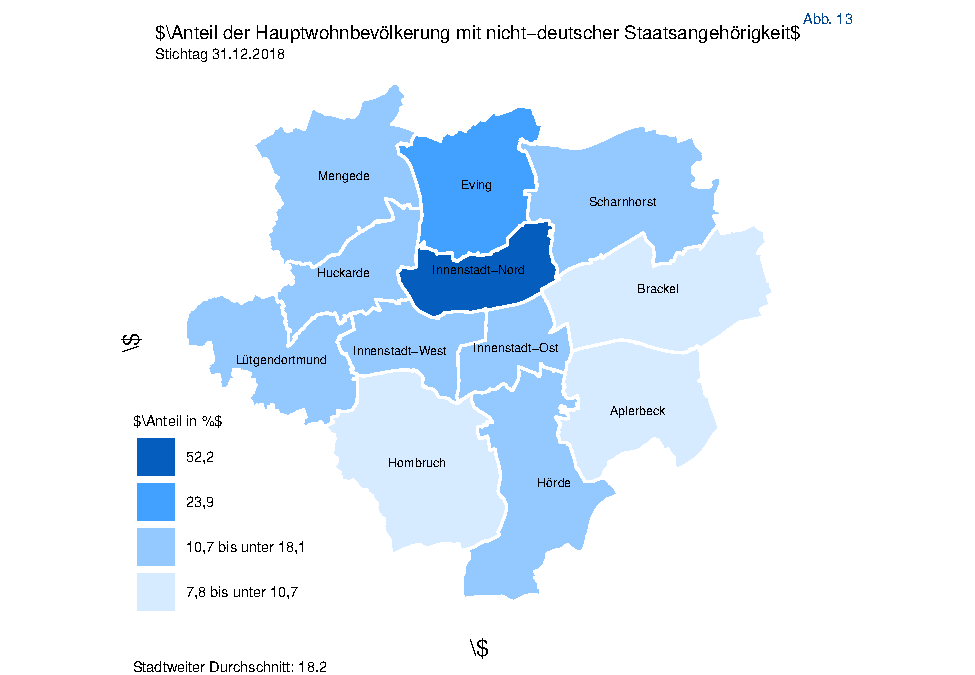
\includegraphics[width=1\linewidth]{2021-03-02_Beispiel_files/figure-latex/Plot map-1} \end{flushright}

Lorem ipsum dolor sit amet, consetetur sadipscing elitr, sed diam nonumy eirmod tempor invidunt ut labore et dolore magna aliquyam erat, sed diam voluptua. At vero eos et accusam et justo duo dolores et ea rebum. Stet clita kasd gubergren, no sea takimata sanctus est Lorem ipsum dolor sit amet. Lorem ipsum dolor sit amet, consetetur sadipscing elitr, sed diam nonumy eirmod tempor invidunt ut labore et dolore magna aliquyam erat, sed diam voluptua. At vero eos et accusam et justo duo dolores et ea rebum. Stet clita kasd gubergren, no sea takimata sanctus est Lorem ipsum dolor sit amet.

\columnbreak

\begin{flushright}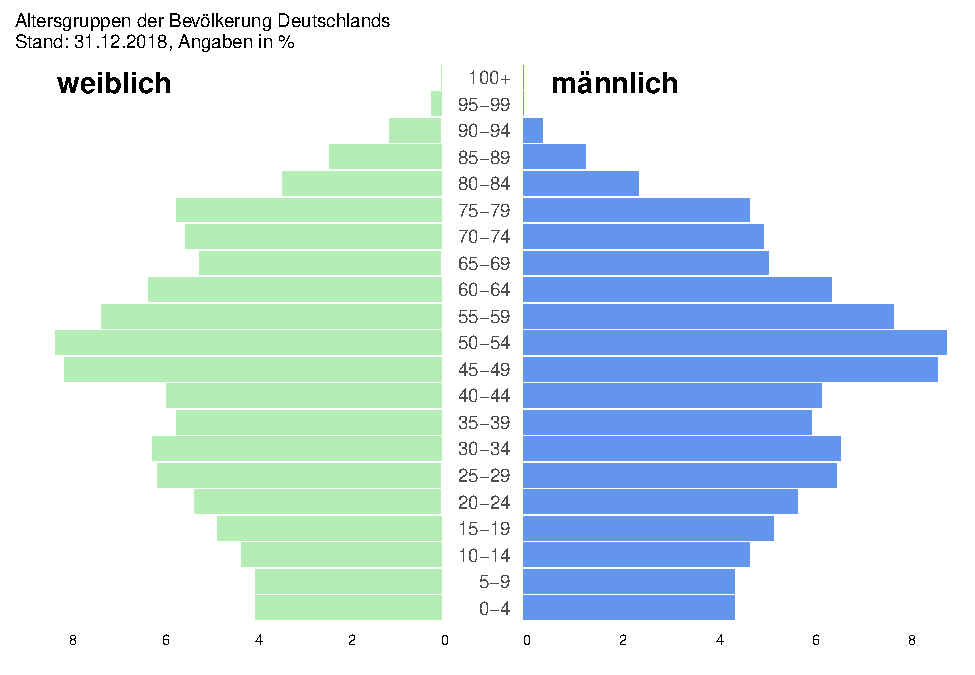
\includegraphics[width=1\linewidth]{2021-03-02_Beispiel_files/figure-latex/plot Pyramide 2-spaltig-1} \end{flushright}

Lorem ipsum dolor sit amet, consetetur sadipscing elitr, sed diam nonumy eirmod tempor invidunt ut labore et dolore magna aliquyam erat, sed diam voluptua. At vero eos et accusam et justo duo dolores et ea rebum. Stet clita kasd gubergren, no sea takimata sanctus est Lorem ipsum dolor sit amet. Lorem ipsum dolor sit amet, consetetur sadipscing elitr, sed diam nonumy eirmod tempor invidunt ut labore et dolore magna aliquyam erat, sed diam voluptua. At vero eos et accusam et justo duo dolores et ea rebum. Stet clita kasd gubergren, no sea takimata sanctus est Lorem ipsum dolor sit amet.

\end {multicols}

Ersichtlich sind auf den ersten Blick folgende To Dos:

\begin{itemize}
\tightlist
\item
  manche Grafiken sind für 2 Spalten ungeeignet -\textgreater{} Entscheidungen welche Grafik in welcher Form wie verwendet wird?
\item
  Maxmierung der Grafikgröße entlang der Spaltenbreite. (Lösung über fig.width, fig.height)
\item
  Skalierung der Grafik Beschriftung anhand der festgelegten Schriftgröße im Gesamtdokument. Hier kann man entweder händisch in ggplot Einstellungen vornehmen oder über das package tikz eine Lösung finden.
\item
  Entscheidung, ob mit Tabellenüberschriften innerhalb der Grafik gearbeitet wird, oder diese über RMarkdown Captions gelöst werden.
\item
  letztendlich macht es aber erst Sinn, wenn die Einbindung der cd Schrift Frutiger gelungen ist.
\end{itemize}

\newpage

\hypertarget{plots-1-spaltig}{%
\subsection{Plots 1 spaltig}\label{plots-1-spaltig}}

Hier eine Ansicht in maximaler Größe

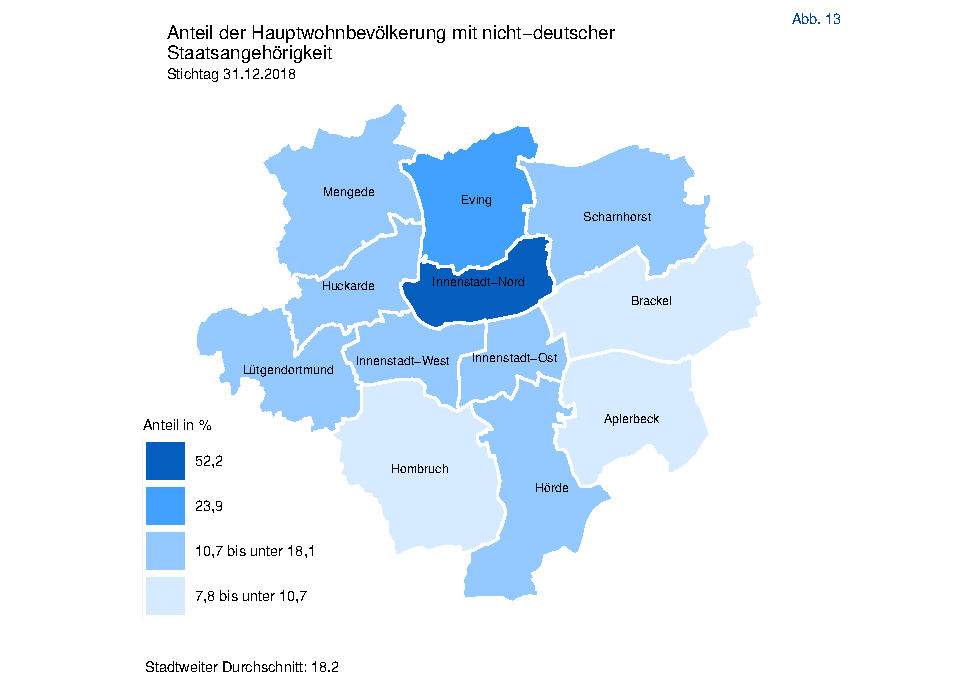
\includegraphics[width=1\linewidth]{2021-03-02_Beispiel_files/figure-latex/Plot map 1 spaltig-1}

\vspace{5mm}

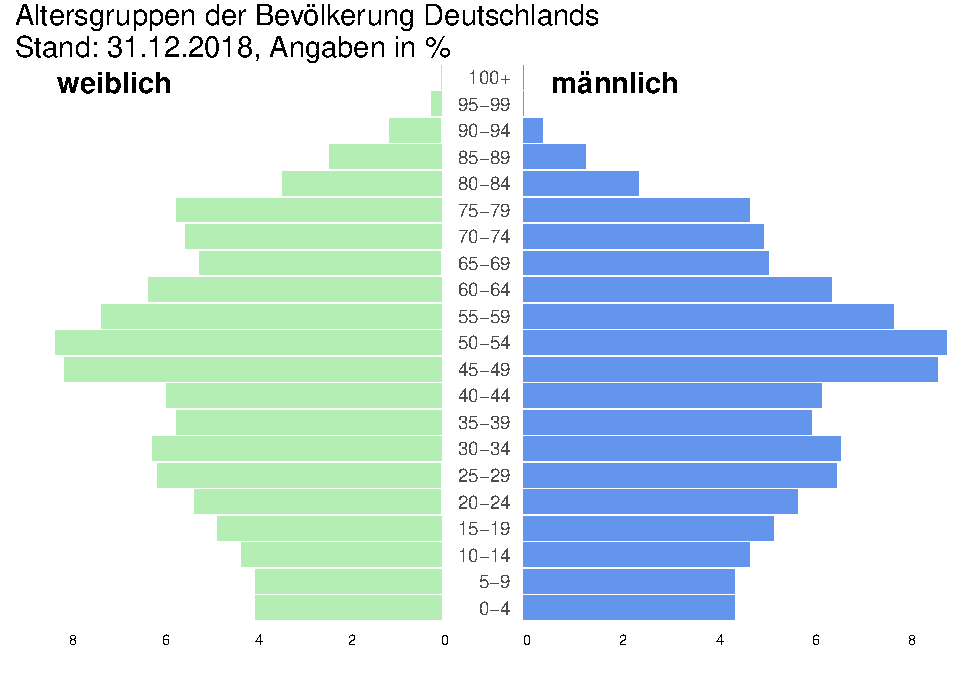
\includegraphics[width=1\linewidth]{2021-03-02_Beispiel_files/figure-latex/plot Pyramide 1 spaltig-1}

\newpage

\hypertarget{tabelle-ganzseitig}{%
\subsection{Tabelle Ganzseitig}\label{tabelle-ganzseitig}}

\begin{table}[!h]

\caption{\label{tab:kable}Stadtbezirk Innenstadt-West: Bevölkerung im Zeitvergleich 2013 bis 2018}
\centering
\resizebox{\linewidth}{!}{
\begin{threeparttable}
\begin{tabular}[t]{lrrrrrrrr}
\toprule
\multicolumn{1}{c}{ } & \multicolumn{2}{c}{2013} & \multicolumn{2}{c}{2017} & \multicolumn{2}{c}{2018} & \multicolumn{1}{c}{2018 / 2013} & \multicolumn{1}{c}{2018 / 2017} \\
\cmidrule(l{3pt}r{3pt}){2-3} \cmidrule(l{3pt}r{3pt}){4-5} \cmidrule(l{3pt}r{3pt}){6-7} \cmidrule(l{3pt}r{3pt}){8-8} \cmidrule(l{3pt}r{3pt}){9-9}
Stadtbezirk Innenstadt-West & Anzahl & \makecell[c]{in \% der \\HWB} & Anzahl & \makecell[c]{in \% der \\HWB} & Anzahl & \makecell[c]{in \% der \\HWB} & \makecell[c]{Anzahl\\} & \makecell[c]{Anzahl\\}\\
\midrule
\addlinespace[0.3em]
\multicolumn{9}{l}{\textcolor[HTML]{044891}{Hauptwohnbevölkerung (HWB)}}\\
\hspace{1em}\hspace{1em}Insgesamt & 52031 & 100.0 & 53323 & 100.0 & 52970 & 100.0 & 939 & -353\\
\addlinespace[0.3em]
\multicolumn{9}{l}{\textcolor[HTML]{044891}{Bevölkerung nach Geschlecht}}\\
\hspace{1em}\hspace{1em}Männlich & 25739 & 49.5 & 26613 & 49.9 & 26441 & 49.9 & 702 & -172\\
\hspace{1em}\hspace{1em}Weiblich & 26292 & 50.5 & 26710 & 50.1 & 26529 & 50.1 & 237 & -181\\
\addlinespace[0.3em]
\multicolumn{9}{l}{\textcolor[HTML]{044891}{Bevölkerung nach Migrationshintergrund}}\\
\hspace{1em}\hspace{1em}Deutsch & 44023 & 84.6 & 43702 & 82.0 & 43362 & 81.9 & -661 & -340\\
\hspace{1em}\hspace{2em}dav. ohne Migrationshintergrund & 35589 & 68.4 & 35419 & 66.4 & 34802 & 65.7 & - & -617\\
\hspace{1em}\hspace{2em}dav. mit Migrationshintergrund & 8434 & 16.2 & 8283 & 15.5 & 8560 & 16.2 & - & 277\\
\hspace{1em}\hspace{1em}Nichtdeutsch (1. Staatsangehörigkeit) & 8008 & 15.4 & 9621 & 18.0 & 9608 & 18.1 & 1600 & -13\\
\addlinespace[0.3em]
\multicolumn{9}{l}{\textcolor[HTML]{044891}{Bevölkerung nach Altersgruppen}}\\
\hspace{1em}\hspace{1em}0 bis unter 3 Jahre & 1238 & 2.4 & 1356 & 2.5 & 1313 & 2.5 & 75 & -43\\
\hspace{1em}\hspace{1em}3 bis unter 6 Jahre & 1102 & 2.1 & 1136 & 2.1 & 1122 & 2.1 & 20 & -14\\
\hspace{1em}\hspace{1em}6 bis unter 18 Jahre & 4123 & 7.9 & 4172 & 7.8 & 4140 & 7.8 & 17 & -32\\
\hspace{1em}\hspace{1em}18 bis unter 25 Jahre & 5729 & 11.0 & 5773 & 10.8 & 5692 & 10.7 & -37 & -81\\
\hspace{1em}\hspace{1em}25 bis unter 35 Jahre & 10667 & 20.5 & 11713 & 22.0 & 11554 & 21.8 & 887 & -159\\
\hspace{1em}\hspace{1em}35 bis unter 50 Jahre & 11095 & 21.3 & 10331 & 19.4 & 10203 & 19.3 & -892 & -128\\
\hspace{1em}\hspace{1em}50 bis unter 65 Jahre & 9259 & 17.8 & 9927 & 18.6 & 9965 & 18.8 & 706 & 38\\
\hspace{1em}\hspace{1em}65 bis unter 80 Jahre & 6294 & 12.1 & 6215 & 11.7 & 6180 & 11.7 & -114 & -35\\
\hspace{1em}\hspace{1em}80 Jahre und älter & 2524 & 4.9 & 2700 & 5.1 & 2801 & 5.3 & 277 & 101\\
\addlinespace[0.3em]
\multicolumn{9}{l}{\textcolor[HTML]{044891}{Bevölkerung nach Familienstand}}\\
\hspace{1em}\hspace{1em}Ledig & 27380 & 52.6 & 28898 & 54.2 & 28697 & 54.2 & 1317 & -201\\
\hspace{1em}\hspace{1em}Verheiratet & 16667 & 32.0 & 16426 & 30.8 & 16319 & 30.8 & -348 & -107\\
\hspace{1em}\hspace{1em}Verwitwet & 3266 & 6.3 & 3107 & 5.8 & 3039 & 5.7 & -227 & -68\\
\hspace{1em}\hspace{1em}Geschieden & 4458 & 8.6 & 4358 & 8.2 & 4290 & 8.1 & -168 & -68\\
\hspace{1em}\hspace{1em}Sonstige & 260 & 0.5 & 534 & 1.0 & 625 & 1.2 & 365 & 91\\
\addlinespace[0.3em]
\multicolumn{9}{l}{\textcolor[HTML]{044891}{Bevölkerung nach Konfession}}\\
\hspace{1em}\hspace{1em}Evangelisch & 13735 & 26.4 & 12829 & 24.1 & 12549 & 23.7 & -1186 & -280\\
\hspace{1em}\hspace{1em}Römisch-katholisch & 14848 & 28.5 & 14298 & 26.8 & 14017 & 26.5 & -831 & -281\\
\hspace{1em}\hspace{1em}Sonstige, ohne Angabe, keine & 23448 & 45.1 & 26196 & 49.1 & 26404 & 49.8 & 2956 & 208\\
\addlinespace[0.3em]
\multicolumn{9}{l}{\textcolor[HTML]{044891}{Bevölkerung mit Nebenwohnsitz}}\\
\hspace{1em}\hspace{1em}Insgesamt & 1060 & 2.0 & 1014 & 1.9 & 969 & 1.8 & -91 & -45\\
\addlinespace[0.3em]
\multicolumn{9}{l}{\textcolor[HTML]{044891}{Bevölkerung nach Haushalten}}\\
\hspace{1em}\hspace{1em}Einpersonenhaushalte & 19985 & 38.4 & 20393 & 38.2 & 20501 & 38.7 & - & 108\\
\hspace{1em}\hspace{1em}(Ehe-)Paare ohne Kind(er) & 14881 & 28.6 & 15027 & 28.2 & 15027 & 28.4 & - & 0\\
\hspace{1em}\hspace{1em}(Ehe-)Paare mit Kind(ern) & 11209 & 21.5 & 11410 & 21.4 & 11193 & 21.1 & - & -217\\
\hspace{1em}\hspace{1em}Alleinerziehende Haushalte & 3147 & 6.0 & 2926 & 5.5 & 2979 & 5.6 & - & 53\\
\hspace{1em}\hspace{1em}Sonstige Mehrpersonenhaushalte & 2809 & 5.4 & 2836 & 5.3 & 2770 & 5.2 & - & -66\\
\hspace{1em}\hspace{1em}Bevölkerung in Haushalten insgesamt & 52031 & 100.0 & 52592 & 98.6 & 52470 & 99.1 & - & -122\\
\addlinespace[0.3em]
\multicolumn{9}{l}{\textcolor[HTML]{044891}{Bevölkerung nach Statistischen Bezirken}}\\
\hspace{1em}\hspace{1em}000-City & 9337 & 17.9 & 9687 & 18.2 & 9707 & 18.3 & 370 & 20\\
\hspace{1em}\hspace{1em}010-Westfalenhalle & 15517 & 29.8 & 15828 & 29.7 & 15863 & 29.9 & 346 & 35\\
\hspace{1em}\hspace{1em}020-Dorstfelder Brücke & 11882 & 22.8 & 12458 & 23.4 & 12362 & 23.3 & 480 & -96\\
\hspace{1em}\hspace{1em}030-Dorstfeld & 15295 & 29.4 & 15350 & 28.8 & 15038 & 28.4 & -257 & -312\\
\bottomrule
\end{tabular}
\begin{tablenotes}
\small
\item[1] Hierzu zählen Lebenspartnerschaft, Lebenspartnerschaft aufgehoben, Lebenspartner verstorben und unbekannt.
\item[2] Sonstige Mehrpersonenhaushalte ohne Paare und ohne Kinder.
\item[3] Seit 2016 werden durch methodische Verbesserungen in der Haushaltegenerierung Personen in Gemeinschaftsunterkünften ausgeschlossen, weshalb die Bevölkerung in Haushalten insgesamt ab 2016 unter 100 \% der HWB liegt. Die Differenz sind die Personen in Gemeinschaftsunterkünften.
\item[4] Durch methodische Verbesserungen (seit 2016) in der Generierung der Daten zum Migrationshintergrund und zu den Haushalten, sind die Daten für einen Zeitvergleich nicht geeignet.
\end{tablenotes}
\end{threeparttable}}
\end{table}

To Dos:

\begin{itemize}
\tightlist
\item
  Fußnoten innerhalb der Tabelle
\item
  Ränder
\item
  Formatierung von Zahlen
\end{itemize}

\newpage

\hypertarget{nuxe4chste-schritte}{%
\section{Nächste Schritte}\label{nuxe4chste-schritte}}

\hypertarget{to-dos-nach-priorituxe4t}{%
\subsection{To Dos nach Priorität}\label{to-dos-nach-priorituxe4t}}

\begin {multicols}{2}

\hypertarget{hoch}{%
\subsubsection{Hoch}\label{hoch}}

Unabdingbar zu lösen:

\begin{itemize}
\tightlist
\item
  Latex Installation auf Verwaltungsrechnern
\item
  Integration von ``frutiger'' Schriftsatz
\end{itemize}

Klärung der Fragen:

\begin{itemize}
\tightlist
\item
  Festlegung gewünschter Produkte und entsprechenden grundlegenden Design Ansprüchen
\item
  Darauf basierend:

  \begin{itemize}
  \tightlist
  \item
    Reicht RMarkdown? Was geht nicht und kann ggf. darauf verzichtet werden?
  \item
    Kann das package ``bookdown'' helfen? siehe auch: Beispiel Tufte
  \item
    Oder ``muss'' Latex umgestiegen werden?
  \end{itemize}
\end{itemize}

Ergebnis: Minimalbeispiel mit Designelementen

\columnbreak

\hypertarget{mittel}{%
\subsubsection{Mittel}\label{mittel}}

\begin{itemize}
\tightlist
\item
  Festlegung von Standardelementen (Tabellen, Grafiken)
\item
  Entwicklung von themes für Standardelemente im Corporate Design
\item
  Lösung für Umschlag und fortgeschrittene Designelemente
\item
  Lösung von Schriftsatz und Grafikskalierung
\end{itemize}

Ergebnis: Minimalbeispiele für Plots/Tabellen als Basis zur Abstimmung zukünftiger Templates

\hypertarget{niedrig}{%
\subsubsection{Niedrig}\label{niedrig}}

\begin{itemize}
\tightlist
\item
  Erstellung der Plots und Tabellen
\item
  Einbindung von Automatisierungsprozessen
\end{itemize}

Ergebnis: Fertige, automatisierte Berichte

\end {multicols}

\end{document}
